%!TEX root = ..\..\dissertation.tex
\section{Co-Development \& Co-Platforming}\label{sec:coDevPltf}
Co-development in systems engineering, product, and production design refers to the simultaneous development or design of two or more systems with some required or anticipated mutual effect on each other, \eg{} a product and the manufacturing system producing it.
Co-development, along with the related concept co-\gls{glos:platforming}, has been gaining footing in research on platforms and reconfigurable manufacturing in particular~\parencite{MichaelisJohannesson,ElMaraghy2015407}.
The end-goal of co-development of products and manufacturing systems, as outlined by~\textcite{MichaelisJohannesson} and shown on \cref{fig:pltfCoDev}, is to achieve platform-based co-development, wherein aligned instantiations of the platforms are simultaneously created as explicit configurations of products and their corresponding manufacturing system.
\begin{figure}[tb]
	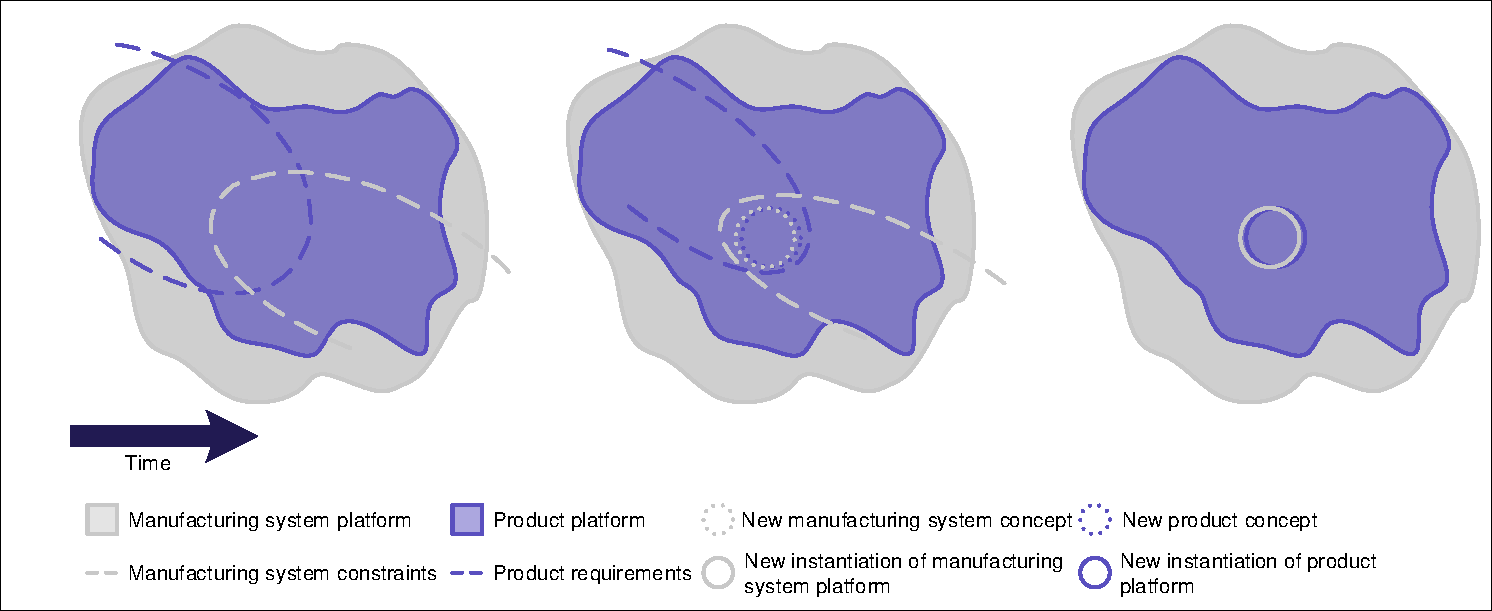
\includegraphics[width=\textwidth, trim=2 2 2 2, clip]{mainmatter/introduction/figures/pltfCoDev.pdf}
	\caption[Platform-based co-development.]
	{Platform-based co-development with new instantiations of the product and manufacturing system platform being developed alongside each other to ensure alignment and compatibility.
	Adapted from \textcite{MichaelisJohannesson}.}\label{fig:pltfCoDev}
\end{figure}

Inconsistencies and lack of communication with regards to platform development as well as misalignment between platforms have proven massive challenges for manufacturers~\parencite{SorensenAPMS2018}.
To address this, and generally improve the synergy between product and manufacturing system development, various approaches to integrate and align the two areas are appearing, such as integrated product and production modelling~\parencite{Michaelis2015203,BRUNOE2018592,BrunoePPModel}, resource modelling and capability matchmaking \parencite{7750724,JARVENPAA201887,dhunganaMarket}, and set-based concurrent engineering utilising platforms \parencite{Levandowski2014,Levandowski01092014,LANDAHL201661}.
Such approaches provide support for a formal way to integrate the work of product and production development teams, ensuring their alignment and compatibility by making it clear which product functions and features are needed, which manufacturing capabilities are available, and how these can be matched, thus facilitating co-development of solutions.